\documentclass{article}


% load package with some of the available options - you may not need this!
\usepackage[framed,numbered,autolinebreaks,useliterate]{mcode}

% something NOT relevant to the usage of the package.
\usepackage{url,textcomp}
\usepackage{graphicx}
\usepackage{epstopdf}
\usepackage{mathtools}
\usepackage{amssymb}
\usepackage{float}
\setlength{\parindent}{0pt}
\setlength{\parskip}{18pt}
\title{\texttt{Machine Learning and Pattern Recognition} Coursework}
\author{Zhen Yi, \texttt{s1563190}}
% //////////////////////////////////////////////////

\begin{document}

\maketitle

\begin{center}
\begin{minipage}{.75\linewidth}
	\color{red}{\hfill\textbf{NOTE --- BEFORE YOU START}\hfill\strut}

    The coursework is formated by \LaTeX{}, if you want a \verb|doc| format copy, please contact me without any hesitation.

\end{minipage}
\end{center}

\section*{Environment for this coursework}

For this coursework, I used \verb|Matlab| as the development tool, and I have some references such as the offical document of \verb|Matlab| ,
the papers and the book which are helpful in theory part.

\medskip

\section*{Solution --- 2 parts}
\subsection*{Part 1}

1.a) For this question, I used command \mcode{histogram(std_tr, 64)}. Please refer to Figuare \ref{fig:11a}. The reason why 64 bins is that although we scaled all the data to 64 bins, we don't change the 
consistency of data. Thus, we still can split the data to 64 bins. \\
This plot tells us the approximate distribution of the standard deviaion of the patches. It looks like that the most of standard devation coverge to zero, thus we can assume that most of the patches are flat patches.

\begin{figure}[H]
    \centering
    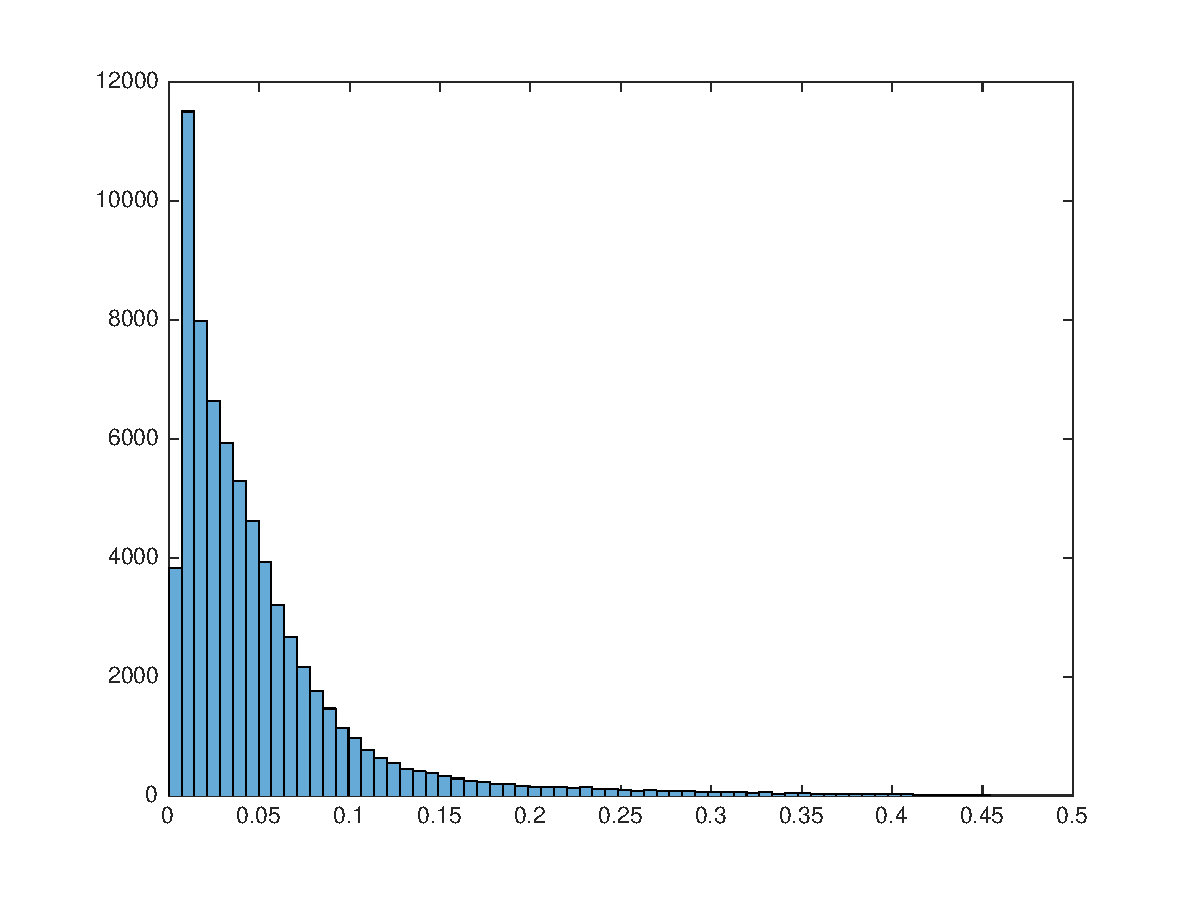
\includegraphics[keepaspectratio=true,width=\linewidth]{./pic/11a.eps} 
    \caption{Histogram(using 64 bins)}
    \label{fig:11a}
\end{figure}


1.b) This question ask us to predict the target pixel, because we have already had the result of standard deviation. We can simply use such result. The meaning of standard deviaion is that if the closer it is to zero, the more flat it is.
Thus, we can use the function \textbf{mean}, which means that most the patch can be seen as flat. Thus, the value of the target pixel closes to the mean of the whole patch.

\lstinputlisting[firstline = 14, lastline = 14]{./t11.m}

1.c) Figure \ref{fig:11c} shows one flat and one non-flat image patch, respectively.

\lstinputlisting[firstline = 16, lastline = 27]{./t11.m}

\begin{figure}[H]
    \centering
    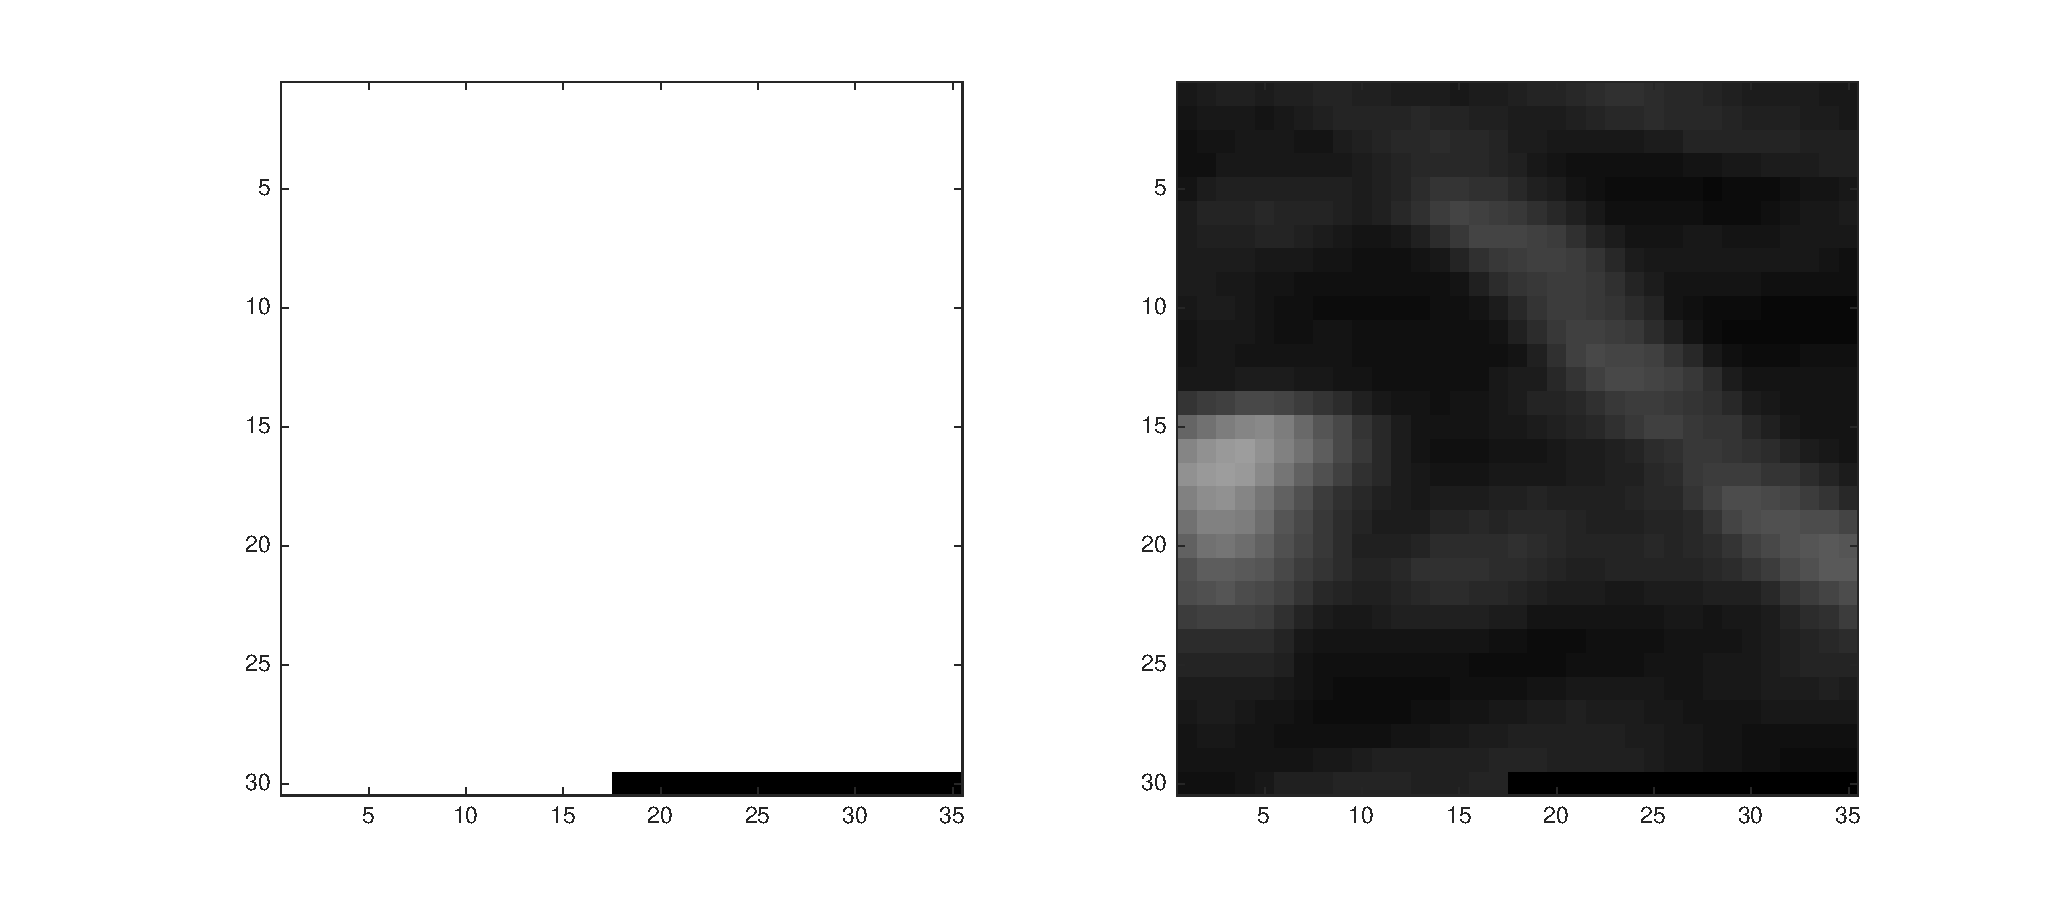
\includegraphics[keepaspectratio=true,width=\linewidth]{./pic/11c.eps}
    \caption{Flat and Non-flat pictures}
    \label{fig:11c}
\end{figure}

Note: Here is the full \verb|Matlab| code for the question 1.
\lstinputlisting{./t11.m}

2.a) Figure \ref{fig:12a} shows that the points cluster near a point (0.25, 0.25, 0.25) which closes to zero. It looks like 
a comet. Most of the points cluster around the such centre point (0.25, 0.25, 0.25), the lower bound and upper bound of this 
body is (0, 0.5]. It also has a tail from (0.5, 1.0). \\
Substantially, it can be seen as positive linear correlation(from (0,0,0) to (1,1,1)). And the part of the points which below (0.5, 0.5, 0.5) is 
more related to the linear correlation than the points which above (0.5, 0.5, 0.5).

\begin{figure}[H]
    \centering
    \includegraphics[keepaspectratio=true,width=\linewidth]{./pic/12a.eps}
    \caption{Subsample}
    \label{fig:12a}
\end{figure}


2.b) The kernel code is \mcode{w = inv(X' * X) * X' * ytr_nf}. We can get the solution of \textbf{w} using X and the vector \textbf{y}:

\begin{center}
    $\log P(y | x, w) = -\frac{1}{2}\log (2\pi \sigma^{2}) - \frac{1}{2\sigma^{2}}(y - w^{T}X)^{2}$\\
    $L (w) = \sum\limits_{i=1}^n (\log P(y_{i}|x_{i}, w))$\\
    $\frac{\partial}{\partial w} L(w) = \frac{\partial}{\partial w} (-\frac{1}{2\sigma^{2}} \sum\limits_{i=1}^n (y_{i}-w^{T}X)^{2})$\\
    $\hat{w} = (X^{T}X)^{-1}X^{T}y$
 \end{center}

\lstinputlisting[firstline = 22, lastline = 25]{./t12.m}

2.c) The linear regression predictor is $y =  X * w$. RMSE of traning data is 0.0506, RMSE of test data is 0.0503. \\
My linear regressor use the closed-form maximum likelihood for weight vector $\vec{w}$, it can work in the simple data sample,
however it may not as powerful as we predicting. Because, it dosen't include any iteration to reduce the error. \\
Now, we need to analyze why RMSE of test data is less than the traning data's. I think, there are more outliers in the traning data.
Thus, such circumstance happens.

\begin{center}
$w = 
 \begin{bmatrix}
     0.4606 \\
     0.5241 \\
     0.0026 
 \end{bmatrix}$
 \end{center}

\begin{figure}[H]
    \centering
    \includegraphics[keepaspectratio=true,width=\linewidth]{./pic/12c.eps}
    \caption{Suface and 3-D plot of test data}
    \label{fig:12c}
\end{figure}

Note: Here is the full \verb|Matlab| code for the question 2.
\lstinputlisting{./t12.m}

3.a) In this question, I used 10-fold cross validation and only map the argument of traning data to function. Figure \ref{fig:13a} shows the 
RMSE of 6 different nbf functions.\\
I have run the \textbf{matlab} program 10 times, and plot them in one diagram. You can see that it is fluctuant. Therefore, we should to choose the 
most stable one from the all 6 possible choice. By observation, I will choose 10 for next problem.

\begin{figure}[H]
    \centering
    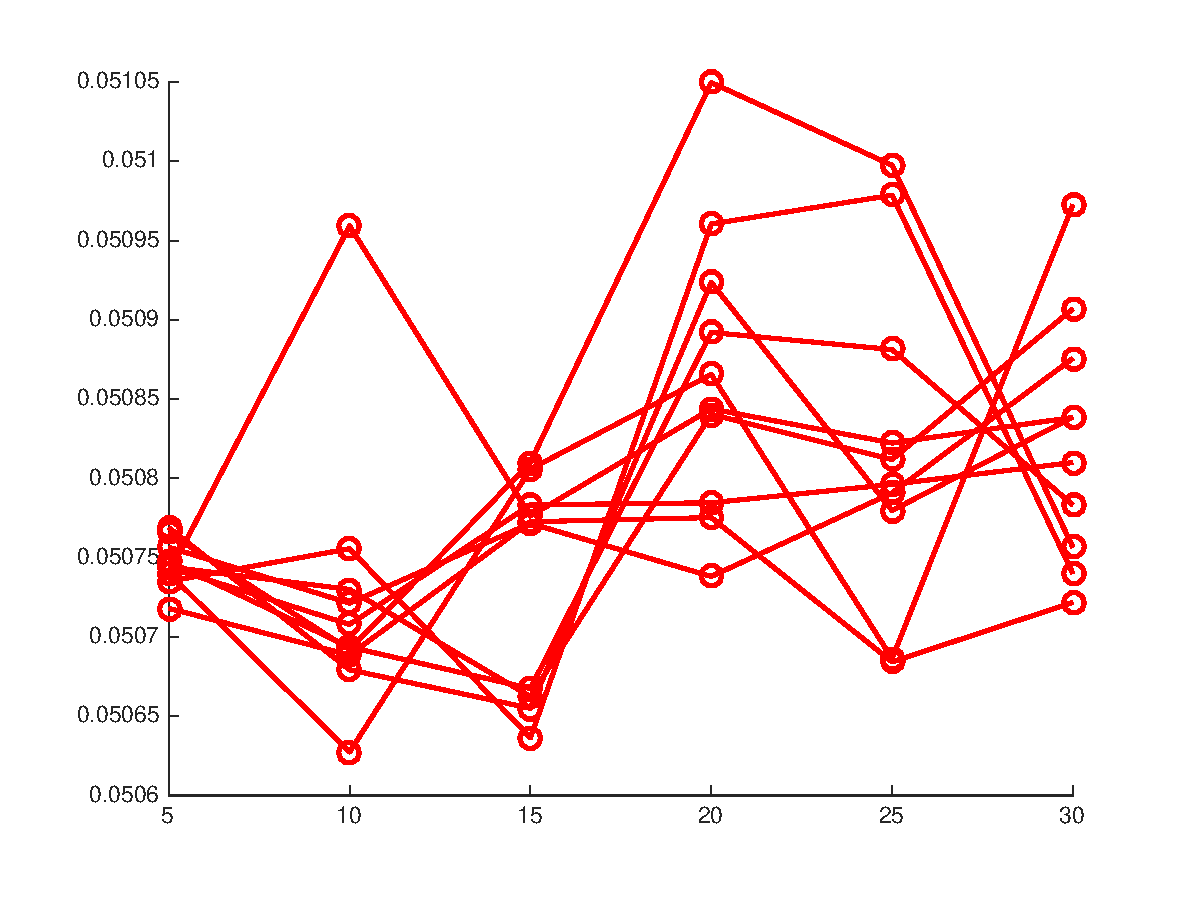
\includegraphics[keepaspectratio=true,width=\linewidth]{./pic/13a.eps}
    \caption{cross-validation RMSE}
    \label{fig:13a}
\end{figure}

Note: Here is the full \verb|Matlab| code for the question 3.a.
\lstinputlisting{./t13.m}

3.b) For this question, the result is better the linear regression, but they are very close. And the method of RBF is totally different from 
linear regression, because of non-linear feature. And the result of test is better than the result of training.

\begin{center}
$RMSE \quad traning = 0.0505$ \\
$RMSE \quad test = 0.0501$ 
 \end{center}

\lstinputlisting{./t13b.m}

4) In this question, we implement a linear regressor with full pixels. The result are :
RMSE of traning data is 0.0371, RMSE of test data is 0.0456. \\
The RMSEs are less than previous result which produced by that linear regressor. The more dimension of the train data is, the 
less RESE we can get. Therefore, we got the better solution.\\
Of course, we can get more features from the larger amount of information. The reason why we use non-flat traning data is that
we should reduce the outliers. For this example, the over-fitting occurs, thus the gap between RMSE of traning data and RMSE of
test data is big.

Note: Here is the full \verb|Matlab| code for the question 4.
\lstinputlisting{./t14.m}

5.a) In this question, I used the well trained MLP to compute both of traning data and test data. The RMSE of traning data is 0.0333, 
the RMSE of test data is 0.0473. The RMSE of traning data is less than such data of linear regression. However, the RMSE of test data is 
greater than such data of linear regression. Only for this example, we can assert that sometimes the performance of NN is not as good as 
linear regression. I guess the reason is that, they used different traning data or the NN is more appropariate traning data, but not test data.
This may cause the over-fitting. Therefore, the result of test data is worse than taht of linear regression.

\lstinputlisting{./t15.m}

5.b) Referring to the table. I report the result of different seed. The gap between the RMSE of traning data and RMSE of test data gets larger.
Because we have tried 5 seeds. We have the different initialization of the corresponding seeds. And the results of the performace are
similiar. So we get the conclusion is that limited data cause the over-fitting problem.

\begin{center}
  \begin{tabular}{l*{4}{c}r}
    Seed         & 2015 & 2016 & 2017 & 2018 & 2019 \\
    \hline
    RMSE train   & 0.0387 & 0.0363 & 0.0346 & 0.0334 & 0.0347 \\
    RMSE test    & 0.0515 & 0.0504 & 0.0515 & 0.0516 & 0.0527 \\
  \end{tabular}
\end{center}

\lstinputlisting{./t15b.m}

6) First of all, I think we should compare the methods in different aspects. We cannot compare them directly, because there exsits some different factors which influenced the results.

\begin{itemize}
  \item Firstly, let we compare the linear regression and RBF network using 2 neighbouring pixels. They have the gap between two RMSEs is very small, which means we can think that they have the
      similiar performance of the result. However, the efficiency of linear regression is much better than the RBF's. Because we do need to choose the number of functions in RBF network. Thus, at least in
      this traning data set, the linear regression is better.
  \item Secondly, in question 4 we used whole image patch to train the linear regressor. And the performance of such regressor is better than the one which used 2 neighbouring pixels(because of less RMSE).
      The reason why that happens is, in my opinion, the amount of the information is larger. Thus, the cost function can get more features to do the gradient descent(although we used the pseudo-method here).
      But the RMSE of test data still higher than the traning one. I think this maybe the problem of over-fitting. It is a serious problem. We should decide the initial parameters carefully.
  \item Thirdly, let we compare neural network with linear regression. In problem 4 and 5, we used all the dimension of the traning data to train the neural network and regressor. Obviously, the method of neural
      network is much complicated than the linear regression. And the serious problem of over-fitting occurrs in the neural network. Thus, the performance of NN is not as good as linear regression.
  \item Finally, there are some different schemes can strengthen the performance of above methods. 
      1) We can use different features of the training data in linear regression. For example, we can use the whole row on
      the left of the predicting pixel and whole columbn on the above of the predicting pixel. The reason is that, we can do the experiment to find which feature is the best one of the problem. 
      2) We can add the prior probability. For example, bayes regression and bayes network.
\end{itemize}

\subsection*{Part 2}

1.a) For this question, the code is been showed as follow. I used the basic method to implement the target which augment a 'bias' weight.
Thus, we can avoid adding extra inputs and outputs to the likelihood function.

\lstinputlisting[firstline = 1, lastline = 4]{./t21.m}

1.b) The follow routine \textbf{t21b} is negative-log-likelihood function:

\lstinputlisting{./t21b.m}

We can use the above function to compute the data we need. Now, let us compare the two different sets. Firstly, the accuracy of traning data is
less than that of test data. It is strange. However, it might be correct because of the features of data or other factors. \\
For the mean log probability(MLP for short), the baseline is $\log{0.5} = -0.693147$. Thus, both the MLP are bigger than the baseline.
And the performance of the test data is still better than the traning one.

\begin{center}
$Accuracy\quad of\quad test = 0.9083$ \\
$Accuracy\quad of\quad training = 0.8344$ \\
$Mean\quad log\quad probability\quad of\quad test= -0.2881$ \\
$Mean\quad log\quad probability\quad of\quad training= -0.4400$
 \end{center}

Here is the full \textbf{matlab} code of 1.b.

\lstinputlisting[firstline = 5, lastline = 44]{./t21.m}

1.c) Here we limited the data to first 100 traning cases. The accuracy and the mean log probability descend dramatically. I think the reason
is that the traning cases is not enough to train the log regressor well. For this example, the first 100 cases cannot represent the general 
feature of the whole data sets.

\begin{center}
$Accuracy\quad of\quad test = 0.7520$ \\
$Mean\quad log\quad probability\quad of\quad test= -inf$ \\
 \end{center}

Here is the full \textbf{matlab} code of 1.c.

\lstinputlisting{./t21c.m}

2.a) For this question, we need to compute the derivatives of both $\textbf{w}$ and $\epsilon$. Such result can be used as the function which compute
the log regression with the label noise.\\
The original function showed as below:

\begin{center}
    $P(y|\textbf{x},\textbf{w},\epsilon) = (1-\epsilon)\sigma(y\textbf{w}^{T}\textbf{x})+\epsilon /2, \qquad y \in \{-1,+1\}$\\
 \end{center}

 Firstly, we should compute the derivative of $\textbf{w}$ :

\begin{center}
    $\mathcal{L}(\textbf{w},\epsilon) = \sum\limits_{n=1}^N \log P(y^{(n)}|x^{(n)},\textbf{w},\epsilon)$ \\ 
    $\nabla_{w}\mathcal{L}(\textbf{w},\epsilon) = \frac{\partial }{\partial w} \sum\limits_{n=1}^N \log P(y^{(n)}|x^{(n)},\textbf{w},\epsilon)$ \\
    $\nabla_{w}\mathcal{L}(\textbf{w},\epsilon) = \frac{\partial y^{(n)}\textbf{w}^{T}x^{(n)}}{\partial w} \frac{\partial }{\partial y^{(n)}\textbf{w}^{T}x^{(n)}} \sum\limits_{n=1}^N \log ((1-\epsilon)\sigma(y^{(n)}\textbf{w}^{T}\textbf{x}^{(n)})+\epsilon /2)$ \\
$\nabla_{w}\mathcal{L}(\textbf{w},\epsilon) = y^{(n)}\textbf{x}^{(n)} \sum\limits_{n=1}^N \left[ \frac{(1-\epsilon)\sigma(y^{(n)}\textbf{w}^{T}x^{(n)})(1-\sigma(y^{(n)}\textbf{w}^{T}x^{(n)}))}{(1-\epsilon)\sigma(y^{(n)}\textbf{w}^{T}\textbf{x}^{(n)})+\epsilon /2}\right]$
 \end{center}

 Secondly, we should compute the derivative of $\epsilon$ :

\begin{center}
    $\mathcal{L}(\textbf{w},\epsilon) = \sum\limits_{n=1}^N \log P(y^{(n)}|x^{(n)},\textbf{w},\epsilon)$ \\
    $\nabla_{\epsilon}\mathcal{L}(\textbf{w},\epsilon) = \frac{\partial }{\partial \epsilon} \sum\limits_{n=1}^N \log P(y^{(n)}|x^{(n)},\textbf{w},\epsilon)$ \\
    $\nabla_{\epsilon}\mathcal{L}(\textbf{w},\epsilon) = \frac{\partial }{\partial \epsilon} \sum\limits_{n=1}^N \log ((1-\epsilon)\sigma(y^{(n)}\textbf{w}^{T}\textbf{x}^{(n)})+\epsilon /2)$ \\
    $\nabla_{\epsilon}\mathcal{L}(\textbf{w},\epsilon) = \sum\limits_{n=1}^N \left[ \frac{\frac{1}{2}-\sigma(y^{(n)}\textbf{w}^{T}x^{(n)})}{(1-\epsilon)\sigma(y^{(n)}\textbf{w}^{T}\textbf{x}^{(n)})+\epsilon /2}\right]$
 \end{center}

Here are the \textbf{matlab} code of the above two derivatives.

\lstinputlisting{./t22f1.m}

\lstinputlisting{./t22f2.m}

Now we can use the routine \textbf{checkgrad.m} to check the derivatives of above two functions. This routine provides
the difference between my gradients and their numerial approximation. However, because of the precision, I found that there might not exsit
the largest difference.

\lstinputlisting{./t22a.m}

2.b) In this problem, we will write the parameter of $\epsilon$ as the result of taking the logistic sigmod of an unconstrained parameter a:

\begin{center}
    $\epsilon = \sigma(a) = \frac{1}{1+exp(-a)}$
\end{center}

Now, we compute the derivative of $a$ :

\begin{center}
    $\mathcal{L}(\textbf{w},a) = \sum\limits_{n=1}^N \log P(y^{(n)}|x^{(n)},\textbf{w},\sigma(a))$ \\
    $\nabla_{a}\mathcal{L}(\textbf{w},a) = \frac{\partial }{\partial a} \sum\limits_{n=1}^N \log P(y^{(n)}|x^{(n)},\textbf{w},\sigma(a))$ \\
    $\nabla_{a}\mathcal{L}(\textbf{w},a) = \frac{\partial }{\partial a} \sum\limits_{n=1}^N \log ((1-\sigma(a))\sigma(y^{(n)}\textbf{w}^{T}\textbf{x}^{(n)})+\sigma(a) /2)$ \\
    $\nabla_{a}\mathcal{L}(\textbf{w},a) = \sum\limits_{n=1}^N \left[ \frac{\sigma(a)(1-\sigma(a))(\frac{1}{2}-\sigma(y^{(n)}\textbf{w}^{T}x^{(n)}))}{(1-\sigma(a))\sigma(y^{(n)}\textbf{w}^{T}\textbf{x}^{(n)})+\sigma(a) /2)}\right]$
 \end{center}

Here is the full \textbf{matlab} code of the function of 2.b.

\lstinputlisting{./t22b.m}

Now, we use the program to compute accuracy and mean log probability(MLP for short). We can get the new result as below:

\begin{center}
    $accuracy = 0.9108$ \\
    $mean\quad log\quad probability = -1.3486$
\end{center}

For this result, we found that the MLP is less than the last problem. And the accuracy is similiar to that problem. We can observe the predicting value of y,
and the value are much more extreme. The reason why that happens is that, I think, we use the constrained parameter to build the sigmoid function of $\epsilon$.\\
On the other hand, because the training data of the problem may not always reliable. Thus, in this problem, we lead into the label noise model. If $s_{n} = 1$ then the
label is chosen with a uniform random choice and ignore the original $\textbf{x}$ features. Therefore, we may guess the correct choice which is not reliable by balance the 
original function with constrained parameter.

Here is the full \textbf{matlab} code of the function of derivative.

\lstinputlisting{./t22f1n.m}

3.a) The largest log-likelihood that any model can given a training set of N binary outcomes equal to the log-likelihood if a model were somehow able to predict every
training label correctly. Thus, it is just 1.

\begin{center}
    Let $w = 0$ in\\
    $\log P(\epsilon,\textbf{w},\log \lambda | data) = \mathcal{L}(\textbf{w},\epsilon) - \lambda \textbf{w}^{T}\textbf{w} + \frac{D}{2}\log \lambda + const$ 
\end{center}

We can get following result:

\begin{center}
    $\log P(\epsilon,0,\log \lambda | data) = \frac{1}{2} + \frac{D}{2}\log \lambda + const$
\end{center}

By questions 1 and 2 in part 2, we have already known the derivative of the $\mathcal{L}(\textbf{w},\epsilon)$ showed as below:

\begin{center}
    $\nabla_{\epsilon}\mathcal{L}(\textbf{w},\epsilon) = \sum\limits_{n=1}^N \left[ \frac{\frac{1}{2}-\sigma(y^{(n)}\textbf{w}^{T}x^{(n)})}{(1-\epsilon)\sigma(y^{(n)}\textbf{w}^{T}\textbf{x}^{(n)})+\epsilon /2}\right]$
\end{center}

Now, we need to solve the extrema of above function:

\begin{center}
    $0 = \sum\limits_{n=1}^N \left[ \frac{\frac{1}{2}-\sigma(y^{(n)}\textbf{w}^{T}x^{(n)})}{(1-\epsilon)\sigma(y^{(n)}\textbf{w}^{T}\textbf{x}^{(n)})+\epsilon /2}\right]$\\
    $\vdots$ \\
    $\sigma(y\textbf{w}^{T}x) = 0$ \\
    $w = 0$
\end{center}

To sum up, the function $\log \lambda$ is the strictly increasing function. Thus, the log-posterior above is globally maximized by setting the weights
to zero and making $\lambda$ infinite.

3.b) For this question, we should implement the function and make the choice of the parameters. 
The parameters of the slice\_sample.m should be decided carefully. For this question, I set all the value of w is 1, and the value of $\epsilon$ and $\log \lambda$ 
are 0.5 and $\log 1$. The width which I set is below 0.2(0.1 for plot the scatter plot). The reason is that, we can get more priciser result.\\
Figure \ref{fig:23b} shows the scatter plot of $\log \lambda$ against $\epsilon$. We can assert that, in this question, our 
posterior beliefs about them are independent. Because we do the simple addition of the two different parts $\mathcal{L}(w,\epsilon)$ and $\frac{D}{2}\log \lambda$.
Therefore they do not affect each other.


\begin{figure}[H]
    \centering
    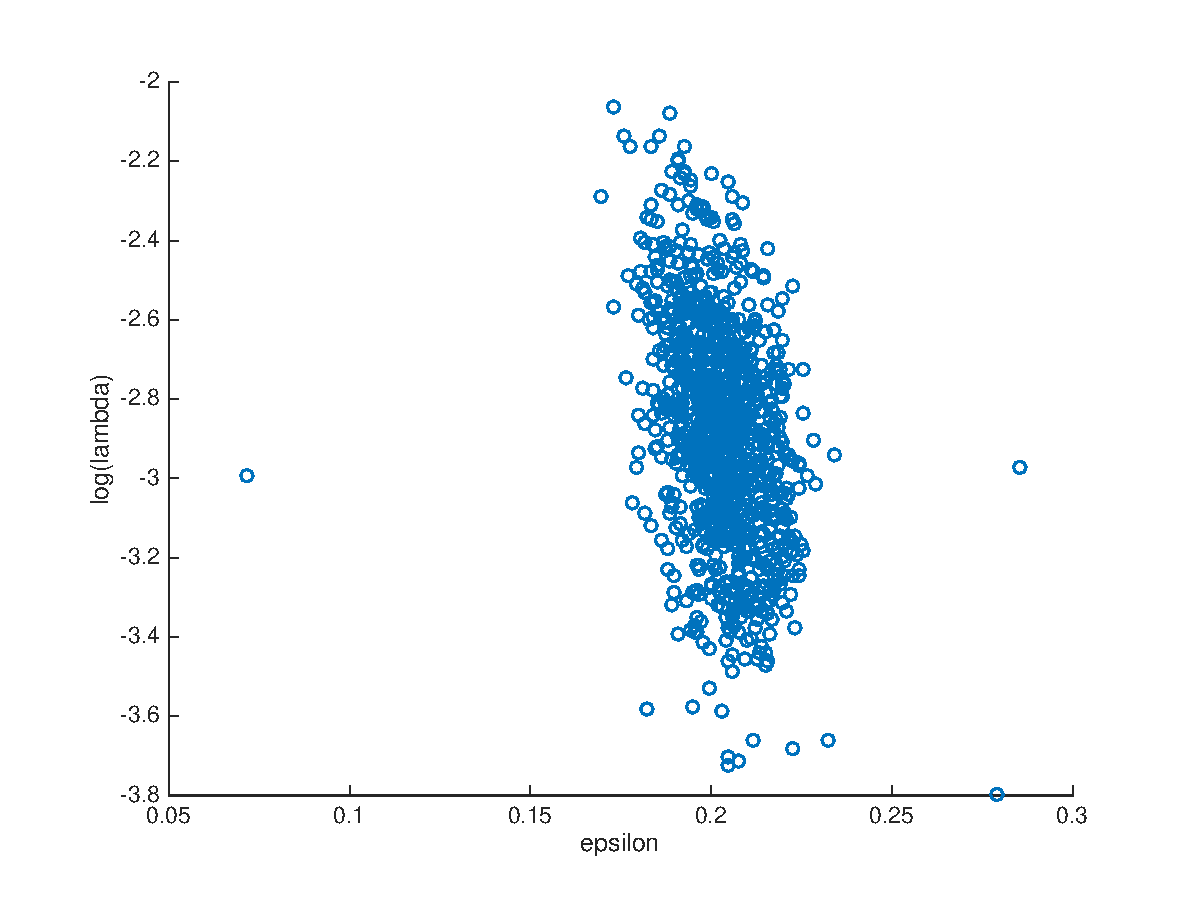
\includegraphics[keepaspectratio=true,width=\linewidth]{./pic/23b.eps}
    \caption{The log(lambda) and epsilon}
    \label{fig:23b}
\end{figure}

\lstinputlisting[firstline = 1, lastline = 11]{./t23.m}

\lstinputlisting{./t23f.m}

3.c) Because of the following estimate:

\begin{center}
    \[ \int f(x)P(x) \,d x \approx \frac{1}{S}\sum\limits_{s=1}^{S}f(x^{(s)}).\] 
\end{center}

Above equation tells us that we should compute all of the prediction by each $\vec{w}$ and do the sum of the results
(for this question, we should compute 1000 results of each sample). Finally, we compute the mean of it.

We can compute the data, and get the accuracy 0.9151. So it is better than the previous model.
Because we compute the mean of the 1000 samples. And some of the prediction of the samples maybe very good. That's why we got
the better result.

Here is the full \textbf{matlab} code of 3.

\lstinputlisting{./t23.m}

\section*{Conclusion}

\begin{description}
	\item[What I have learned]
        Basically, I learned how to use \textbf{matlab} to write some simple routines.
        Futhur more, the topic of comparing the different models and how to set the initial guess data are all very important.
        The ability to compare the two or more models is what I have grasped.
	\item[Where should I make the improvement]
        I have to say that this is the most tough coursework which I have seen. I work hard and spend so much time on it. However, 
        the methods which I have used are not good enough. And some of the princples cannot be undertood deeply by me. Thus, I should do more
        on the theoritical part. Ann then, I think I can report better. 
        The best practice is that I should study more resource both on papers and examples. 
\end{description}

\end{document}
